\documentclass[12pt]{scrartcl}
\usepackage{graphicx}
\usepackage{amsmath}

\newcommand{\RN}[1]{%
  \textup{\uppercase\expandafter{\romannumeral#1}}%
}

\begin{document}
\title{Interaction of a "cold plume" with a subduction zone}
\subtitle{Semester Thesis}
\author{Florian Frei}

\maketitle

\newpage

\tableofcontents

\newpage

\section{Motivation}
Seismological measurements from Columbia shown in figure \ref{fig:seism_data} suggests that an rare geological scenario is happening. The geophysical community agrees that what is probably happening is the rare case where a "cold plume" is detached from the lithosphere and interacts with the subduction plate beneath it. In this project the goal is to use a simplified subduction model to simulate what longterm tendencies could develop and investigate the sensitivity on the parameters for the individual scenarios.
\begin{figure}
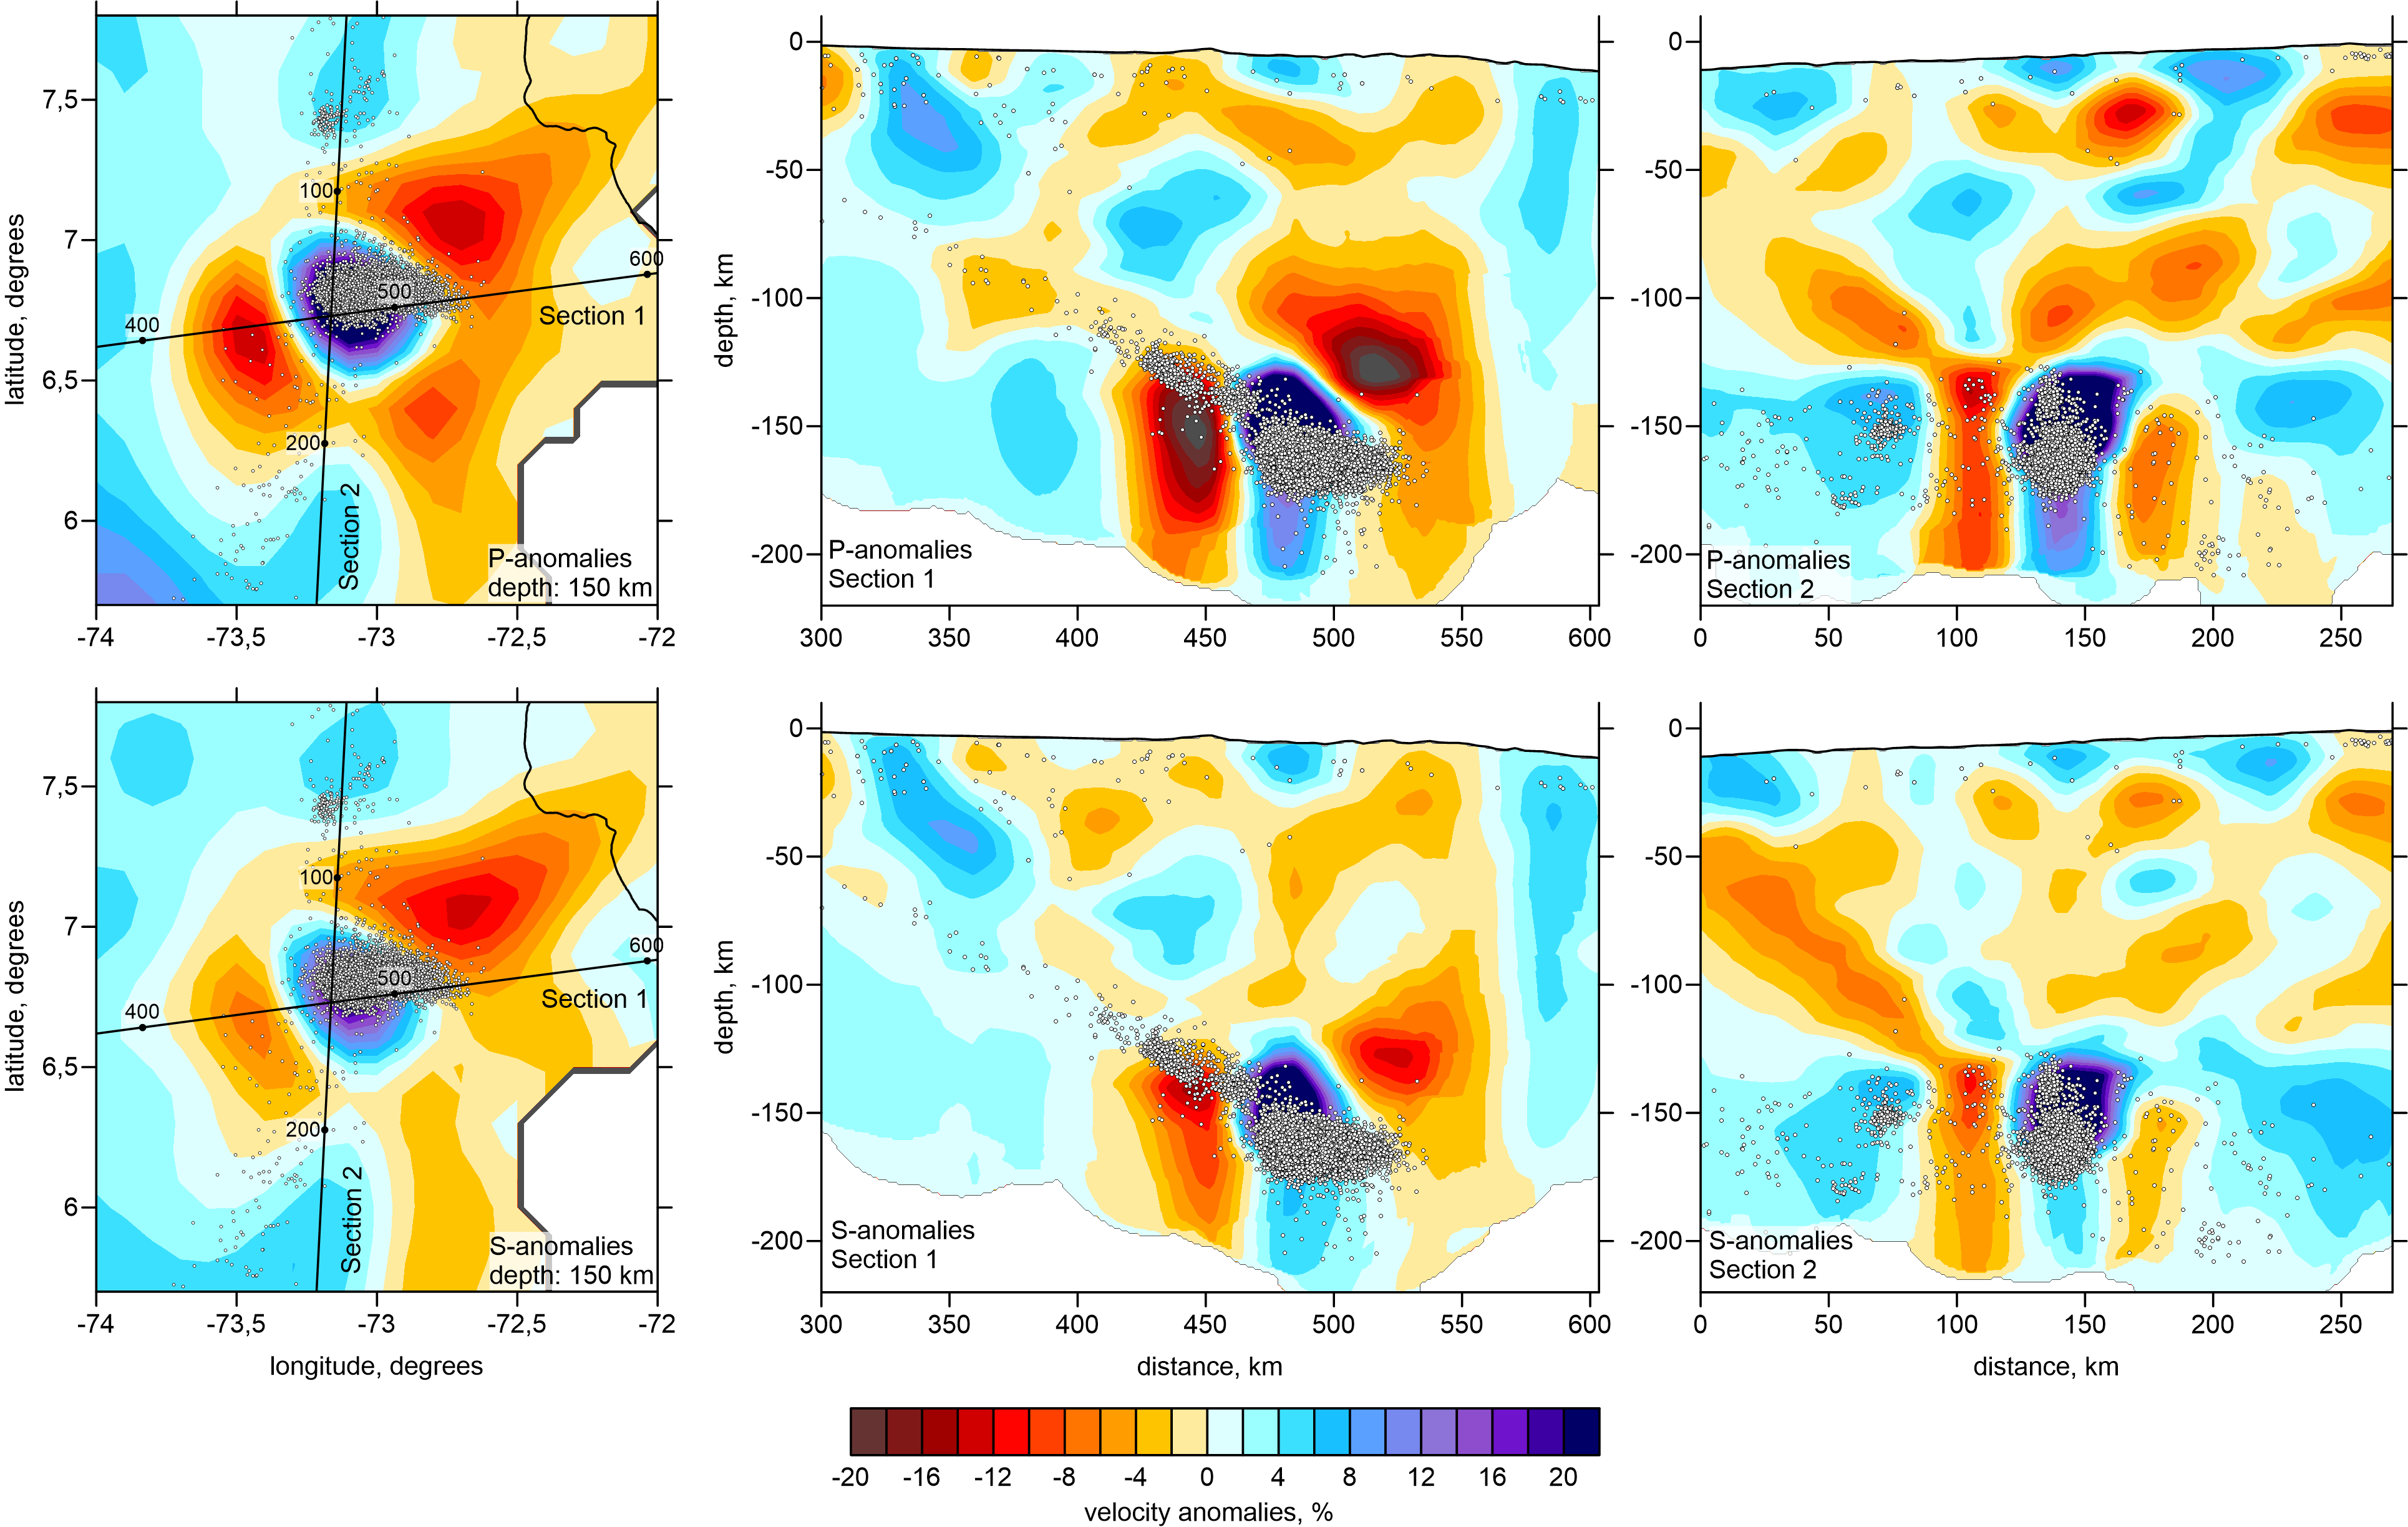
\includegraphics[scale=0.45]{deep_anomaly_hor_ver.png}
\label{fig:seism_data}
\end{figure}

\section{Geophysical Model}
The skill how to correctly model geophysics for a numerical simulation is to vast that it could fit into a single book much less into a simple report. A good starting point which is essential to understand this project is the book "Introduction to Numerical Geodynamic Modelling" \cite{gerya2009introduction} from Taras Gerya.
\subsection{Physical Equations}

empirical rheological relation

\begin{equation}
\dot{\gamma}=A_D h^m (\sigma_d)^n\exp\left( -\frac{E_a+V_a P}{RT} \right)
\label{eq:emprheolrel}
\end{equation}

isotropic, incompressible materials
\begin{equation}
\sigma_{\RN{2}} = 2 \eta_{eff}\dot{\epsilon}_{\RN{2}}
\end{equation}

\section{Model setup}

\section{Implementation}
\section{Results}
\section{Conclusion}

\nocite{vargas2013tearing}
\nocite{gerya2009introduction}




\newpage

\bibliographystyle{plain}
\bibliography{references}


\end{document}

